% Title page and colophon
\begin{titlepage}
\thispagestyle{empty}
\begin{tikzpicture}[remember picture,overlay]
  \fill[guigrey] (current page.north west) rectangle ([yshift=-104mm]current page.north east);
  \fill[okgreen] ([yshift=-104mm]current page.north west) rectangle ([xshift=70mm,yshift=-106.5mm]current page.north west);
  \fill[okamber] ([xshift=70mm,yshift=-104mm]current page.north west) rectangle ([xshift=140mm,yshift=-106.5mm]current page.north west);
  \fill[okblue]  ([xshift=140mm,yshift=-104mm]current page.north west) rectangle ([yshift=-106.5mm]current page.north east);
  \node[anchor=north west,text=white,font=\sffamily\bfseries\fontsize{13}{15}\selectfont,align=left]
    at ([xshift=30mm,yshift=-30mm]current page.north west) {GUIDEBOOK\enspace{\mdseries\color{white!70!guigrey}$\cdot$\enspace Version \AgenticVersion}};
  \node[anchor=north west,text=white,font=\sffamily\bfseries\fontsize{52}{56}\selectfont]
    at ([xshift=29mm,yshift=-40mm]current page.north west) {AgenticTO};
  \node[anchor=north west,text=white!88!guigrey,font=\sffamily\fontsize{15}{20}\selectfont,align=left,text width=150mm]
    at ([xshift=30mm,yshift=-66mm]current page.north west)
    {Agent-assisted, certified 3D topology optimization on one GPU:\\ the workspace, the tool contract and the release record};
  \node[anchor=north,inner sep=0] at ([yshift=-122mm]current page.north)
    {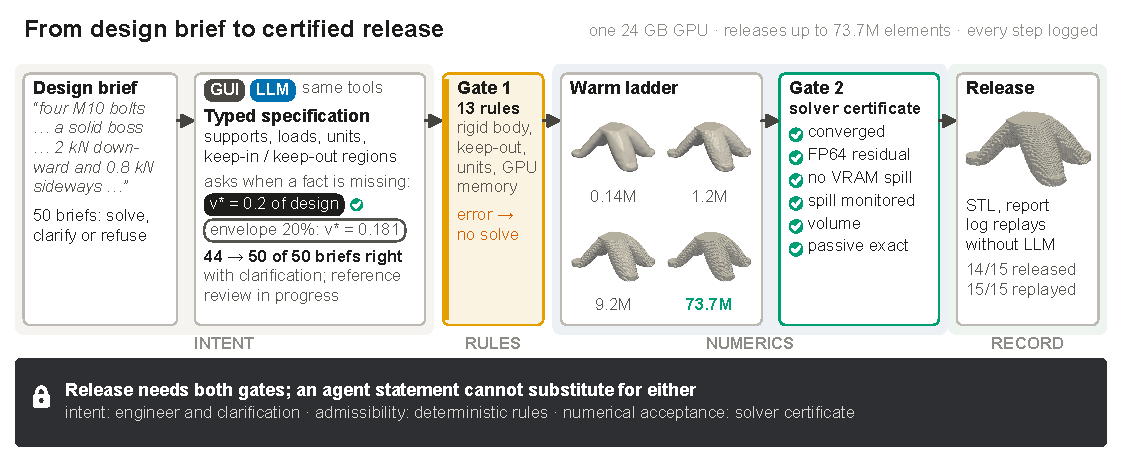
\includegraphics[width=160mm]{graphical_abstract_art.pdf}};
  \node[anchor=north west,font=\sffamily,align=left,text width=150mm] at ([xshift=30mm,yshift=-200mm]current page.north west)
    {{\fontsize{14}{18}\selectfont\bfseries Shaoliang Yang \quad Jun Wang}\\[2mm]
     {\color{muted}Department of Mechanical Engineering, Santa Clara University}\\[9mm]
     {\small\color{muted}Companion to the paper}\\[1mm]
     {\small\itshape\rmfamily \papertitle}};
  \node[anchor=south west,font=\sffamily\small\color{muted},align=left,text width=150mm]
    at ([xshift=30mm,yshift=22mm]current page.south west)
    {October 2026\hfill Software version \AgenticVersion, spec schema \texttt{agentto.spec/v0}};
\end{tikzpicture}
\end{titlepage}

% ---- colophon ----
\thispagestyle{empty}
\vspace*{\fill}
{\small\sffamily
\textbf{AgenticTO Guidebook}\\
Version \AgenticVersion, October 2026. Describes AgenticTO \AgenticVersion\ (Python package \code{agentto}) and the
specification schema \code{agentto.spec/v0}.

\medskip
\textbf{Authors.} Shaoliang Yang and Jun Wang, Department of Mechanical Engineering, Santa Clara University,
500 El Camino Real, Santa Clara, CA 95053, USA. Correspondence: Jun Wang, \href{mailto:jwang22@scu.edu}{jwang22@scu.edu}.

\medskip
\textbf{Software.} The application code, the 50-brief task suite with its adjudicated reference readings, the saved
agent outputs and tool logs, the numerical result records, the generators of the tables and data figures, and the
\code{voxfem} solver that AgenticTO runs on (BSD 3-Clause; Chapter~\ref{ch:install}) are available at \url{\repourl}.

\medskip
\textbf{How this book is made.} The reference tables for the specification schema, the rules, the tools, the certificate,
the schedules, the command-line flags, the HTTP endpoints, the keyboard map and the script catalogue are generated from
the source code by \code{docs/guidebook/gen\_tables.py}, so they match the code they describe. Every screenshot comes from a
real session recorded by \code{scripts/guide\_shots.py}, which drives the workspace with real clicks and keystrokes.
Numbers about performance and accuracy are taken from the paper or from the result files it cites, never measured
again for this book; each such number is marked with its claim identifier from \code{results/claims\_ledger.md}, for
example \claim{C3.1}.

\medskip
\textbf{Scope.} AgenticTO is research software. A certificate in this book means a set of numerical acceptance checks
on a stated computation. It is not a structural safety assessment, and a released design needs further engineering
analysis before anything is built from it.

\medskip
\textbf{Typography.} Set in XCharter, Helvetica and Inconsolata. Colours follow the paper's figures: green for a passing
check, vermillion for a failure, blue for the agent, amber for the rule gate, dark grey for the workspace.
}
\clearpage
